\documentclass[../generics]{subfiles}

\begin{document}

\chapter{Basic Operation}\label{rqm basic operation}

\IndexDefinition{requirement machine}
\lettrine{I}{nformally speaking, a requirement machine} collects generic requirements in a manner amenable to automated reasoning. Previously in this book, you saw a specific style of hand-written proof in the examples motivating generic signature queries and requirement minimization. Starting from a generic signature, each step of our proof would derive a conclusion from a requirement appearing either in the signature itself or a protocol referenced by a conformance requirement. In the final step we would either conclude with the result of our generic signature query, or show that some requirement was redundant. This is essentially what a requirement machine does, except as you will see, in a sense we actually pre-compute all possible proofs simultaneously.

This chapter shows how requirement machines are constructed, leaving the rest for later, but in the interest of not being completely abstract we will also preview some of the key ideas from subsequent chapters here.
\begin{center}
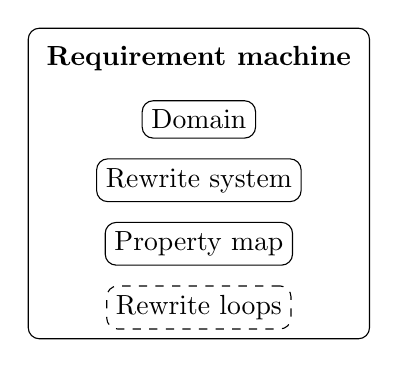
\begin{tikzpicture}
\tikzstyle{data} = [rounded corners, draw=black, text centered]

\matrix [data, row sep=0.25cm]
{
\node (RequirementMachine) {\textbf{Requirement machine}}; \\
\node (Domain) [data] {Domain}; \\
\node (RewriteSystem) [data] {Rewrite system}; \\
\node (PropertyMap) [data] {Property map}; \\
\node (RewriteLoops) [data, dashed] {Rewrite loops}; \\
};

\end{tikzpicture}
\end{center}
\index{domain}%
\index{rewrite system}%
\index{property map}%
\index{rewrite loop}%
\index{minimal requirement}%
Concretely, a requirement machine consists of these four parts:
\begin{itemize}
\item A \emph{domain}, which is either a list of generic parameters or a list of protocols.
\item A \emph{rewrite system}, comprised of \emph{rewrite rules}. The rewrite system simplifies \emph{terms}, which among other things is how we compute reduced types (Section~\ref{reducedtypes}).
\item A \emph{property map}, which collects certain rewrite rules in a form suitable for efficient lookup. The property map helps implement the aforesaid generic signature queries (Section~\ref{genericsigqueries}).
\item Optionally, a set of \emph{rewrite loops}, which describe relations among rewrite rules. Rewrite loops aren't needed for queries, so we only record them when computing minimal requirements (Section~\ref{minimal requirements}).
\end{itemize}
Requirement machines come in four varieties:
\begin{enumerate}
\item \textbf{Generic signature}, where we build a requirement machine from the requirements of an existing generic signature to answer generic signature queries.
\item \textbf{Generic signature minimization}, where we build a requirement machine from user-written requirements in order to compute the minimal requirements for a new generic signature.
\item \textbf{Protocol component}, where we build a requirement machine from an already-known requirement signature of each protocol in a component.
\item \textbf{Protocol component minimization}, where we build a requirement machine from user-written requirements in a protocol component in order to compute a requirement signature for each protocol in the component.
\end{enumerate}
Note that we have all four combinations of domain and ``purpose.'' In case (1) and (2) above, the domain is a list of generic parameters. In case (3)~and~(4), the domain is a list of protocols in a protocol component (which will be introduced shortly). In case (1)~and~(3), our goal is to build a requirement machine and use its rewrite system and property map, so we don't record rewrite loops. In case (2)~and~(4), we're also computing a list of minimal requirements, so we \emph{do} record rewrite loops. Let's now take a closer look at each of these four possibilities.

\paragraph{Generic signature}
\index{generic signature query}%
\IndexDefinition{rewrite context}%
\index{rewrite rule}%
\index{rule builder}%
\IndexDefinition{local rule}%
\IndexDefinition{imported rule}%
To answer a generic signature query, we first build a requirement machine from the requirements of an existing generic signature. Requirement machines for generic signature queries are owned by a singleton object, the \emph{rewrite context}. One responsibility of the rewrite context is maintaining a table mapping generic signatures to requirement machines. The implementation of each generic signature query begins by requesting a requirement machine for the given signature, which consults the mapping and creates a new requirement machine if necessary. Figure~\ref{rqm flowchart generic signature} shows the key steps in building a requirement machine from a generic signature:
\begin{itemize}
\item First, we lower the generic signature's requirements to \emph{rewrite rules}; these become the \emph{local rules} of our new requirement machine.

\item We also collect the rewrite rules from each protocol component referenced by the signature; these are the \emph{imported rules}. We'll discuss imported rules when we introduce protocol components in the next section.

\item Once we have the initial set of rewrite rules, we run the \index{completion}\emph{completion procedure} (Chapter~\ref{completion}). Completion introduces new local rules which are ``consequences'' of existing rules. As you will learn, completion makes our rewrite system \emph{confluent}, which has desirable theoretical consequences.

\item After completion, we construct the property map (Chapter~\ref{propertymap}). The property map is a compact representation of the conformance, superclass, layout and concrete type requirements imposed on each type parameter.

\item Property map construction might introduce new local rules, which possibly breaks confluence, in which case completion must run again; completion and property map construction must both be repeated until neither adds any more rules.

\item Once constructed, a requirement machine becomes immutable for the remainder of its lifetime.

\end{itemize}
\Index{getRequiredProtocols()@\texttt{getRequiredProtocols()}}%
\index{term}%
After all that, we can answer generic signature queries about our generic signature's type parameters. For example, the \texttt{getRequiredProtocols()} generic signature query first lowers the given type parameter to a term, then simplifies the term using the rewrite system, and finally looks up the simplified term in the property map. The property map entry immediately stores a list of protocols this type parameter conforms to.

\begin{figure}\captionabove{Building a requirement machine for an existing generic signature}\label{rqm flowchart generic signature}
\begin{center}
\begin{tikzpicture}[node distance=0.75cm]
\tikzstyle{data} = [rounded corners, draw=black, text centered]
\tikzstyle{stage} = [rectangle, draw=black, text centered]
\tikzstyle{arrow} = [->,>=stealth]

\node (MinimalRequirements) [data] {Minimal requirements};
\node (ImportedRules) [data, right=of MinimalRequirements] {Imported rules};
\node (RuleBuilder) [stage, below=of MinimalRequirements] {\vphantom{p}Rule builder};
\node (Completion) [stage, below=of RuleBuilder] {Completion};
\node (PropertyMap) [stage, below=of Completion] {Property map construction};
\node (RequirementMachine) [data, below=of PropertyMap] {Requirement machine};

\draw [arrow] (MinimalRequirements) -- (RuleBuilder);
\draw [arrow] (ImportedRules) |- (RuleBuilder);
\draw [arrow] (RuleBuilder) -- (Completion);
\draw [arrow] (Completion) -- (PropertyMap);
\draw [arrow] (PropertyMap.east) -- ++ (0.5, 0) |- (Completion);

\draw [arrow] (PropertyMap) -- (RequirementMachine);

\end{tikzpicture}
\end{center}
\end{figure}

\index{request evaluator}
The lazy construction of a requirement machine for a generic signature is similar to a request evaluator request (Section~\ref{request evaluator}), but it does not actually rely on the request evaluator infrastructure. An equivalent of a request cycle can also happen here: we invoke a generic signature query against some generic signature, and in the middle of constructing this requirement machine, we invoke another generic signature query against the same signature. This is extremely difficult to hit in practice, so for simplicity it is reported as a fatal error which immediately exits the compiler.
\begin{figure}\captionabove{Building a requirement machine for a new generic signature}\label{rqm flowchart generic signature minimization}
\begin{center}
\begin{tikzpicture}[node distance=0.75cm]
\tikzstyle{data} = [rounded corners, draw=black, text centered]
\tikzstyle{stage} = [rectangle, draw=black, text centered]
\tikzstyle{arrow} = [->,>=stealth]

\node (DesugaredRequirements) [data] {Desugared requirements};
\node (ImportedRules) [data, right=of DesugaredRequirements] {Imported rules};
\node (RuleBuilder) [stage, below=of DesugaredRequirements] {\vphantom{p}Rule builder};
\node (Completion) [stage, below=of RuleBuilder] {Completion};
\node (PropertyMap) [stage, below=of Completion] {Property map construction};

\node (Minimization) [stage, below=of PropertyMap] {Rewrite system minimization};

\node (RequirementMachine) [data, below=of Minimization] {Requirement machine};
\node (RequirementBuilder) [stage, right=of Minimization] {Requirement builder};
\node (MinimalRequirements) [data, below=of RequirementBuilder] {Minimal requirements};

\draw [arrow] (DesugaredRequirements) -- (RuleBuilder);
\draw [arrow] (ImportedRules) |- (RuleBuilder);
\draw [arrow] (RuleBuilder) -- (Completion);
\draw [arrow] (Completion) -- (PropertyMap);
\draw [arrow] (PropertyMap.east) -- ++ (0.5, 0) |- (Completion);

\draw [arrow] (PropertyMap) -- (Minimization);
\draw [arrow] (Minimization) -- (RequirementMachine);
\draw [arrow] (Minimization) -- (RequirementBuilder);
\draw [arrow] (RequirementBuilder) -- (MinimalRequirements);

\end{tikzpicture}
\end{center}
\end{figure}

\paragraph{Generic signature minimization}
\index{inferred generic signature request}%
\index{abstract generic signature request}%
\index{minimal requirement}%
\index{desugared requirement}%
We get here if evaluating the \Request{inferred generic signature request} or \Request{abstract generic signature request}. These requests build new generic signatures with a multiple-step process summarized in Figure \ref{inferred generic signature request figure}~and~\ref{abstract generic signature request figure} of Chapter~\ref{building generic signatures}. The last step in both flows was ``requirement minimization,'' a magical black box transforming desugared requirements into minimal requirements. Figure~\ref{rqm flowchart generic signature minimization} gives you a sneak peek inside this black box. While similar to the previous case of building a machine for generic signature queries, there are several important differences:
\begin{itemize}
\item First of all, we start with a list of desugared requirements, rather than minimal requirements. (The rewrite system does not actually care if the requirements fed into the rule builder are minimal or not.)
\item As completion runs, it discovers relations between existing rules and the new rules it adds; these relations are now recorded and represented as rewrite loops.
\item After the rewrite system and property map have been built, the minimization algorithm processes the rewrite loops to find a minimal subset of rewrite rules which completely describe the rewrite system. This is the topic of Chapter \ref{rqm minimization}.
\index{requirement builder}%
\item The \emph{requirement builder} converts these minimal rewrite rules back into requirements. A new generic signature is then built from the original list of generic parameters that were given to the request, together with these newly-computed minimal requirements. This is explained in Section~\ref{requirement builder}.
\end{itemize}

At this point, we have our new generic signature, and we could simply discard the new requirement machine. While that would be correct, if the frontend were to issue a generic signature query against the new generic signature, we would have to build a whole new requirement machine from these now-minimal requirements. This is quite common; for example, after building the generic signature of a function declaration, we often go on to type check the function's body, which might perform many generic signature queries against this same signature.

To avoid wasting time rebuilding the same requirement machine again later, we ask the rewrite context if it already had a requirement machine for the new generic signature. If it has one, then our new requirement machine is truly not needed anymore, and we can tear it down and reclaim the memory used by its data structures. However, if we built a generic signature we have not seen before, we \emph{install} the new requirement machine into the rewrite context's table.

\IndexFlag{disable-requirement-machine-reuse}%
Of course it is worth asking if a requirement machine built from desugared user-written requirements has the same observable behavior as one built from minimal requirements. The answer is ``almost always,'' but there are several important exceptions. If any of the below three conditions hold, the new requirement machine is always discarded and never installed, because we cannot guarantee the same results as if we had rebuilt a fresh machine from the output of the minimization algorithm:
\begin{itemize}
\item If any of the user-written requirements were invalid, the invalid requirements will not appear in the final generic signature, even though the corresponding rewrite rules are part of our \index{rewrite system}rewrite system.
\item As you will see in Chapter~\ref{completion}, \index{completion}completion can also fail if the original requirements are too complex. In this case the final generic signature will have no requirements, but the rewrite system will include all rewrite rules computed up to the point of failure.
\item There is an edge case involving conformance requirements and concrete types that we will talk about in Chapter~\ref{concrete conformances}.
\end{itemize}
 The \texttt{-disable-requirement-machine-reuse} frontend flag forces the rewrite context to always just discard the requirement machine after minimization. If you're lucky enough to discover a new scenario not covered by one of the above cases, then this flag might address the problem; it would certainly make for an interesting bug report!

\paragraph{Protocol component}
\index{protocol component}%
A requirement machine for a protocol component is built in a similar way to Figure~\ref{rqm flowchart generic signature}. We take with the requirement signature of each protocol in the component, build rewrite rules, run completion, and construct the property map. Protocol component machines are never directly used for queries; we only issue queries against generic signature machines. Instead, protocol component machines only have one purpose in life: to have their rewrite rules imported into other requirement machines.
\eject
The rule builder here converts the requirements of the requirement signature into rules, and it also introduces a rule for each associated type declaration in the protocol as well. You will see how these rules work in Chapter~\ref{symbols terms rules}.

\index{serialized module}%
\index{requirement signature}%
\index{main module}%
Typically, protocol component requirement machines are created for protocols that were deserialized from another module, where the requirement signatures were previously computed and serialized as well. For protocols in the main module (that is, written in source) we use the fourth and final kind of requirement machine to compute their requirement signatures first; this requirement machine is then installed in the rewrite context so that those rules can be imported later. However, just as the generic signature minimization requirement machine cannot be installed under some circumstances, the same edge cases can force us to discard the protocol component minimization requirement machine instead of installing it, in which case we will build a new protocol component requirement machine from the requirement signatures we just built.

\paragraph{Protocol component minimization}
\index{structural requirements request}%
\index{type alias requirements request}%
\index{requirement signature request}%
\index{associated type declaration}%
The final variety of requirement machine is created by the \Request{requirement signature request} to compute new requirement signatures for the protocol declarations in the main module. The flow is similar to Figure~\ref{rqm flowchart generic signature minimization}. As you saw in Chapter~\ref{building generic signatures}, we compute the desugared requirements for a requirement signature by evaluating the \Request{structural requirements request} and \Request{type alias requirements request}. These requirements are then fed into the rule builder. Just as with the protocol component requirement machine, we introduce rewrite rules for the protocol's associated types as well.

\section{Protocol Components}\label{protocol component}

\index{requirement signature}%
\index{associated conformance requirement}%
\index{conformance requirement}%
A requirement machine is constructed from an initial list of requirements. To understand the type parameters described by these requirements, we need to look inside the protocols named by the conformance requirements as well. Each one of these protocols can declare associated types and state further requirements on those associated types; hence we also look at the requirement signature of each protocol, and recursively consider any protocols named by \emph{those} requirements, and so on. (Recall from Section~\ref{associated conformances} that the conformance requirements of a protocol's requirement signature are called associated conformance requirements).

TODO: mention domain

\paragraph{Derived requirements}
There is a link between the protocol dependency graph and the \index{derived requirement}derived requirements formalism. Define a relation \index{$\prec$}\index{$\prec$!z@\igobble|seealso{reachability relation}}$\prec$ between protocols, where $\texttt{P}\prec\texttt{Q}$ if $G_\texttt{P}\vDash\ConfReq{T}{Q}$ for some type parameter \texttt{T}; that is, $\texttt{P}\prec\texttt{Q}$ means that we can derive a conformance requirement mentioning \texttt{Q} starting from the requirements of \texttt{P}. Now, this conformance requirement has a conformance path, to which we can apply our graph homomorphism and get a path from \texttt{P} to \texttt{Q}. Thus, $\texttt{P}\prec\texttt{Q}$ can also be understood as the reachability relation in the protocol dependency graph. In Chapter~\ref{rqm basic operation}, we make use of this fact when building the rewrite system for a generic signature, by pulling in the requirements of protocols reachable via the protocol dependency graph.

\index{protocol dependency graph}%
\IndexDefinition{protocol dependency set}%
To formalize this, we refer back to the idea of the protocol dependency graph from Section~\ref{recursive conformances}. The vertices in this graph are protocol declarations, and edges are given by associated conformance requirements. (You might want to review that section first, together with the definition of a directed graph from Section~\ref{type parameter graph}.) We can take the set of protocols named by the conformance requirements in our original list, and compute the transitive closure of this set in the protocol dependency graph to obtain the \emph{protocol dependency set} for our requirement machine.

\IndexDefinition{transitive closure}%
\begin{definition} Given a directed graph $(V,\, E)$ and an initial set of vertices $S\subseteq V$, the \emph{transitive closure} of $S$ in $(V,\, E)$ is the set of vertices reachable via a path originating from an element of $S$. This includes trivial paths, so $S$ is contained in its own transitive closure.
\end{definition}

\begin{listing}\captionabove{Protocol component demonstration}\label{protocol component listing}
\begin{Verbatim}
protocol P {
  associatedtype A: Q
  associatedtype B: R
}

protocol Q {
  associatedtype A: P
  associatedtype B: S
}

protocol R {
  associatedtype A: T
}

protocol S {
  associatedtype A: T
}

protocol T {}
\end{Verbatim}
\end{listing}

Let's look at the protocol dependency graph for Listing~\ref{protocol component listing}:
\begin{quote}
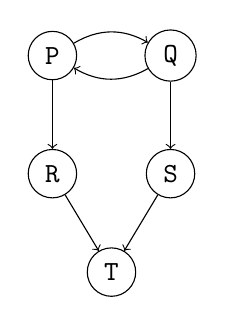
\begin{tikzpicture}[node distance=1.5cm]
\tikzstyle{protocol} = [circle, draw=black, text centered]

\node (P) [protocol] {\texttt{P}};
\node (Q) [protocol, right of=P] {\texttt{Q}};
\node (R) [protocol, below of=P] {\texttt{R}};
\node (S) [protocol, below of=Q] {\texttt{S}};
\node (T) [protocol] at (0.75, -2.75) {\texttt{T}};

\path [->] (P) edge [bend left] (Q)
           (Q) edge [bend left] (P)
           (P) edge (R)
           (Q) edge (S)
           (R) edge (T)
           (S) edge (T);
\end{tikzpicture}
\end{quote}
This suggests that in order to compute the requirement signature for \texttt{P} we first need the requirement signature of \texttt{Q} (and \texttt{R}, \texttt{S} and \texttt{T}). But, by the same line of reasoning, to build the requirement signature of \texttt{Q}, we first need the requirement signature of \texttt{P}! That is, the protocol dependency set of \texttt{P} contains \texttt{Q}, and the protocol dependency set of \texttt{Q} contains \texttt{P}. To resolve this conundrum, we must actually build the requirement signatures of \texttt{P} and \texttt{Q} \emph{simultaneously}. We can formalize this with a little more graph theory.

We say that \texttt{P} and \texttt{Q} are \emph{strongly connected} if either $\texttt{P}=\texttt{Q}$, or $\texttt{P}\prec\texttt{Q}$ and $\texttt{Q}\prec\texttt{P}$. This is an \index{equivalence relation}equivalence relation, and every protocol belongs to exactly one \index{strongly-connected component}\emph{strongly connected component}, which is a list of one or more protocols. The protocols in a strongly-connected component all refer to each other via associated conformance requirements.

In our example, we have two strongly connected components; \verb|P| is in a component by itself, while \verb|Q| and \verb|R| belong to the other component. These three associated conformance requirements are recursive by our definition, however $\AssocConf{Self.C}{P}$ in protocol \verb|R| is not:
\begin{itemize}
\item $\AssocConf{Self.A}{P}$ of protocol \verb|P|;
\item $\AssocConf{Self.B}{R}$ of protocol \verb|Q|;
\item $\AssocConf{Self.D}{Q}$ of protocol \verb|R|.
\end{itemize}

\IndexDefinition{strongly-connected component}%
\index{directed graph}%
\index{vertex}%
\index{edge}%
\begin{definition}
A \emph{strongly-connected component} in a directed graph $(V,\, E)$ is a set of vertices $S\subseteq V$ such that every pair of vertices in $S$ is connected by a path in $(V,\, E)$.
\end{definition}
\IndexDefinition{protocol component}
Indeed, this is why we have protocol \emph{component} machines and protocol \emph{component} minimization machines, and not \emph{protocol} machines and \emph{protocol} minimization machines. A protocol component is a strongly-connected component of the protocol dependency graph. If a component contains multiple protocols, our formalism must reason about the combined requirements of these protocols together as a single unit.

\index{directed graph}
\IndexDefinition{directed acyclic graph}
\index{DAG|see {directed acyclic graph}}
The strongly-connected components of a directed graph define a new directed graph. Each strongly-connected component becomes a vertex, and two distinct components are connected by an edge if the original graph has an edge joining some vertex of the source component with another vertex in the destination component. An important property of the graph of strongly-connected components is that it cannot have cycles, because the existence of a cycle in the original graph necessarily collapses all the vertices visited by the cycle into a single component. A directed graph without cycles is called a \emph{directed acyclic graph}.

If we take the protocol dependency graph and form the directed acyclic graph of strongly-connected components, we get the \emph{protocol component graph}. In our example, \texttt{P} and \texttt{Q} belong to the same protocol component; all other protocols belong to singleton components, giving us this protocol component graph:
\begin{quote}
\begin{tikzpicture}[node distance=1.5cm]
\tikzstyle{protocol} = [rectangle, draw=black, text centered]

\node (PQ) [protocol] {$(\texttt{P},\, \texttt{Q})$};
\node (R) [protocol, below left of=P] {(\texttt{R})};
\node (S) [protocol, below right of=P] {(\texttt{S})};
\node (T) [protocol, below right of=R] {(\texttt{T})};

\path [->] (PQ) edge (R)
           (PQ) edge (S)
           (R) edge (T)
           (S) edge (T);
\end{tikzpicture}
\end{quote}

We lazily construct a protocol component requirement machine for each vertex of the protocol component graph. When building each of these requirement machines, we first import the rewrite rules from all other downstream machines, a recursive process which builds those machines first if necessary, and so on. Since the protocol component graph is acyclic, this must eventually terminate.

Thus, to build the protocol component requirement machine for $(\texttt{P},\, \texttt{Q})$, we must first build the requirement machines for $(\texttt{R})$ and $(\texttt{S})$, and each one of those necessitates building the requirement machine for $(\texttt{T})$. The requirement machines for $(\texttt{R})$ and $(\texttt{S})$ import the rules from $(\texttt{T})$, and the requirement machine for $(\texttt{P},\, \texttt{Q})$ import the rules from $(\texttt{R})$ and $(\texttt{S})$. However, we must take care not to import the rules for $(\texttt{T})$ \emph{twice} when building $(\texttt{P},\, \texttt{Q})$, because there are two distinct paths from $(\texttt{P},\, \texttt{Q})$ to $(\texttt{T})$.

\index{local rule}%
To avoid importing duplicate rules, we only ever import the \emph{local} rules of downstream requirement machines; that is, we compute the transitive closure of $(\texttt{P},\, \texttt{Q})$ in the protocol component graph, and import the local rules from each requirement machine in this transitive closure. Intuitively, each imported rule is the local rule of some downstream requirement machine, so by visiting all downstream machines and collecting their local rules, we get the full set of necessary rules without duplicates.

\IndexDefinition{protocol dependencies request}%
\index{requirement signature request}%
\index{structural requirements request}%
\index{rewrite context}%
\index{successor}%
All of this is managed by the rewrite context. We don't actually construct the entire protocol dependency graph ahead of time, because we don't want to deserialize every protocol in every imported module. Instead, everything is done lazily. First of all, the protocol dependencies of a protocol---that is, the successors of a vertex in the protocol dependency graph---are obtained by evaluating the \Request{protocol dependencies request}, which computes the result as follows:
\begin{itemize}
\item If the protocol is declared inside the main module, we evaluate the \Request{structural requirements request} and collect the protocols mentioned by any conformance requirements in the resulting list.

\item If the protocol is part of a serialized module, we evaluate the \Request{requirement signature request} (the protocol's requirement signature was already computed and serialized) and again collect the protocols mentioned by any conformance requirements in the resulting list.
\end{itemize}

The rewrite context builds the strongly-connected components of the protocol dependency graph using Tarjan's algorithm \cite{tarjan}. This algorithm maintains four temporary values for each vertex in the directed graph---two integers denoted ``index'' and ``low link,'' and two flags, ``visited'' and ``on stack.'' Upon completion it assigns a ``component ID'' integer to each vertex. In the rewrite context, this is represented by a table mapping protocol declarations to \textbf{protocol nodes}, where each protocol node stores these four temporary values together with the assigned component ID. The rewrite context also maintains the ``next component ID,'' which is one greater than the last component ID assigned, together with a stack of protocol declarations.

\IndexDefinition{Tarjan's algorithm}%
\index{successor}%
\begin{algorithm}[Tarjan's algorithm]
Takes a vertex \texttt{V} as input, and computes its component ID, where two vertices have the same component ID if and only if they belong to the same strongly connected component.
\begin{enumerate}
\item (Invariant) Ensure the ``visited'' flag of \texttt{V} is false. If it is true, we either assigned a component ID already, or we have an invalid re-entrant call.
\item (Initialize) Set the ``index'' and ``low link'' of \texttt{V} to the next component ID. Set the ``on stack'' and ``visited'' flags of \texttt{V} to true. Push \texttt{V} on the stack and increment the next component ID.
\item (Visit successors) For each outgoing edge of \texttt{V}:
\begin{enumerate}
\item Let $\texttt{V}^\prime$ be the destination vertex of this edge.
\item If the ``visited'' flag of $\texttt{V}^\prime$ is false: recursively invoke the algorithm on $\texttt{V}^\prime$. Once the recursive call returns, set the ``low link'' of \texttt{V} to the minimum of the ``low link'' of \texttt{V} and $\texttt{V}^\prime$.
\item Otherwise, if the ``visited'' \emph{and} ``on stack'' flags of $\texttt{V}^\prime$ are true: set the ``low link'' of \texttt{V} to the minimum of the ``low link'' of \texttt{V} and the ``index'' of $\texttt{V}^\prime$.
\end{enumerate}
\item (Root?) If the ``low link'' and ``index'' of \texttt{V} are not equal, return.
\item (Pop) Pop a vertex $\texttt{V}_0$ from the stack (which must be non-empty at this point) and clear the ``on stack'' flag of $\texttt{V}_0$.
\item (Assign) Set the component ID of $\texttt{V}_0$. FIXME
\item (Repeat) If the stack is not empty, go back to Step~5.
\end{enumerate}
\end{algorithm}

\index{protocol declaration}%
An important property of Tarjan's algorithm is that it is \emph{incremental}; if we haven't assigned a component ID to a vertex, the vertex must belong to a strongly-connected component distinct from all others formed so far. Invoking the algorithm finds all other vertices belonging to this strongly-connected component, and assigns it a new component ID. This allows us to work with an incomplete protocol dependency graph; any future protocol declarations deserialized during the execution of the frontend job must always belong to hitero-unseen components (but those components may depend on existing components).

Having assigned each protocol a component ID, the rewrite context builds a mapping from component IDs to \textbf{protocol components}. Each protocol component stores a list of protocol declarations together with a lazily-initialized requirement machine. This requirement machine is either a protocol component requirement machine, or a protocol component minimization requirement machine; which one depends on whether we're building requirement signatures for these protocols, or if we already have them.

\index{imported rule}%
\index{rule builder}%
Finally, we have the algorithm used by the rule builder to collect imported rules when building any of the four varieties of requirement machine. This algorithm computes the transitive closure of a set of protocols, collects the requirement machines for each protocol's component, and imports the local rules from each requirement machine.
\begin{algorithm}[Importing rules from protocol components]\label{importing rules}
As input, takes a list \texttt{P} of protocols appearing on the right hand side of our conformance requirements. As output, returns a list of imported rules.
\begin{enumerate}
\item Initialize a worklist and add all the elements of \texttt{P}.
\item Initialize \texttt{S} to a set of visited protocols, initially empty.
\item Initialize \texttt{M} to an empty set of requirement machines (compared by pointer equality).
\item If the worklist is empty, go to Step~10.
\item Otherwise, remove the next protocol $p$ from the worklist. If $p$ is already in \texttt{S}, go back to Step~4, otherwise add $p$ to \texttt{S}.
\item Look up the protocol component of $p$, and create its requirement machine if necessary.
\item If this requirement machine is not already in \texttt{M}, add it to \texttt{M}.
\item Add each protocol dependency of $p$ to the worklist.
\item Go back to Step~4.
\item Initialize \texttt{R} to an empty list of rewrite rules.
\item For each requirement machine $m\in\texttt{M}$, add the local rules of $m$ to \texttt{R}.
\item Return \texttt{R}.
\end{enumerate}
\end{algorithm}

\section{Debugging Flags}

\IndexFlag{analyze-requirement-machine}
\texttt{-analyze-requirement-machine}

\IndexFlag{dump-requirement-machine}
\texttt{-dump-requirement-machine}

\IndexFlag{debug-requirement-machine}
\IndexTwoFlag{debug-requirement-machine}{timers}
\IndexTwoFlag{debug-requirement-machine}{protocol-dependencies}
\texttt{-debug-requirement-machine}

Passing the \texttt{-debug-requirement-machine=timers} frontend flag allows you to watch the rewrite context forming protocol components and importing rules as it builds requirement machines. Listing~\ref{rqm trace listing} shows an example program and the output of running the compiler with this flag.

\begin{listing}\captionabove{Example program and \texttt{-debug-requirement-machine=timers} output}\label{rqm trace listing}
\begin{Verbatim}
func f<T: Sequence, U: Sequence>(_: T, _: U)
    where T.Element == U.Element {}

func g<T: Collection>(_: T) {}

func h<T: BinaryInteger>(_: T) {}
\end{Verbatim}
\begin{Verbatim}[fontsize=\scriptsize,numbers=none]
+ started InferredGenericSignatureRequest @ example.swift:1:7
| + started getRequirementMachine() [ Sequence ]
| | + started getRequirementMachine() [ IteratorProtocol ]
| | + finished getRequirementMachine() in 21us: [ IteratorProtocol ]
| + finished getRequirementMachine() in 34us: [ Sequence ]
+ finished InferredGenericSignatureRequest in 126us: <T, U where T : Sequence, U : Sequence,
                                                      T.Element == U.Element>
+ started InferredGenericSignatureRequest @ example.swift:4:7
| + started getRequirementMachine() [ Collection ]
| | + started getRequirementMachine() [ Comparable ]
| | | + started getRequirementMachine() [ Equatable ]
| | | + finished getRequirementMachine() in 7us: [ Equatable ]
| | + finished getRequirementMachine() in 13us: [ Comparable ]
| + finished getRequirementMachine() in 136us: [ Collection ]
+ finished InferredGenericSignatureRequest in 123us: <T where T : Collection>
+ started InferredGenericSignatureRequest @ example.swift:6:7
| + started getRequirementMachine() [ BinaryInteger ]
| | + started getRequirementMachine() [ CustomStringConvertible ]
| | + finished getRequirementMachine() in 7us: [ CustomStringConvertible ]
| | + started getRequirementMachine() [ Hashable ]
| | + finished getRequirementMachine() in 7us: [ Hashable ]
| | + started getRequirementMachine() [ Numeric ]
| | | + started getRequirementMachine() [ AdditiveArithmetic ]
| | | + finished getRequirementMachine() in 7us: [ AdditiveArithmetic ]
| | | + started getRequirementMachine() [ ExpressibleByIntegerLiteral ]
| | | | + started getRequirementMachine() [ _ExpressibleByBuiltinIntegerLiteral ]
| | | | + finished getRequirementMachine() in 10us: [ _ExpressibleByBuiltinIntegerLiteral ]
| | | + finished getRequirementMachine() in 21us: [ ExpressibleByIntegerLiteral ]
| | + finished getRequirementMachine() in 93us: [ Numeric ]
| | + started getRequirementMachine() [ Strideable ]
| | | + started getRequirementMachine() [ SignedNumeric ]
| | | + finished getRequirementMachine() in 53us: [ SignedNumeric ]
| | + finished getRequirementMachine() in 59us: [ Strideable ]
| | + started getRequirementMachine() [ RandomAccessCollection ]
| | | + started getRequirementMachine() [ BidirectionalCollection ]
| | | + finished getRequirementMachine() in 229us: [ BidirectionalCollection ]
| | + finished getRequirementMachine() in 372us: [ RandomAccessCollection ]
| + finished getRequirementMachine() in 744us: [ BinaryInteger ]
+ finished InferredGenericSignatureRequest in 792us: <T where T : BinaryInteger>
+ started getRequirementMachine() <τ_0_0>
+ finished getRequirementMachine() in 7us: <τ_0_0>
\end{Verbatim}
\end{listing}

\section{Source Code Reference}\label{rqm basic operation source ref}

Key source files:
\begin{itemize}
\item \SourceFile{lib/AST/RequirementMachine/}
\end{itemize}
The Requirement Machine implementation is private to \texttt{lib/AST/}. The remainder of the compiler interacts with it indirectly, through the generic signature query methods on \texttt{GenericSignature} (Section~\ref{genericsigsourceref}) and the various requests for building new generic signatures (Section~\ref{buildinggensigsourceref}).

\subsection*{The Rewrite Context}

Key source files:
\begin{itemize}
\item \SourceFile{lib/AST/RequirementMachine/RewriteContext.h}
\item \SourceFile{lib/AST/RequirementMachine/RewriteContext.cpp}
\end{itemize}

\IndexSource{rewrite context}
\apiref{rewriting::RewriteContext}{class}
A singleton which constructs requirement machines and uniquely-allocates symbols and terms. The \texttt{ASTContext::getRewriteContext()} method returns the unique instance of the rewrite context.
\begin{itemize}
\item \texttt{getRequirementMachine(CanGenericSignature)} returns a requirement machine for the given generic signature, creating one first if necessary.
\IndexSource{protocol component}
\IndexSource{strongly-connected component}
\item \texttt{getRequirementMachine(ProtocolDecl *)} returns a requirement machine for the protocol component which contains the given protocol, creating one first if necessary.
\IndexSource{protocol dependency graph}
\item \texttt{getProtocolComponentImpl()} is a private helper which returns the strongly-connected component of the protocol dependency graph which contains the given protocol.
\IndexSource{Tarjan's algorithm}
\item \texttt{getProtocolComponentRec()} actually implements Tarjan's algorithm for computing strongly-connected components.
\item \texttt{isRecursivelyConstructingRequirementMachine()} has two overloads, taking a generic signature or protocol component. They return true if we are currently constructing a requirement machine for this generic signature or protocol component. This is used as a cycle-breaking hack in associated type inference, since otherwise re-entrant construction triggers an assertion in the compiler.
\item \texttt{installRequirementMachine()} has two overloads, taking a generic signature minimization or  protocol component minimization requirement machine. They record it as the canonical requirement machine for the generic signature or protocol component that was just built.
\end{itemize}

\index{generic signature}
\apiref{GenericSignature}{class}
See also Section~\ref{genericsigsourceref}.
\begin{itemize}
\item \texttt{getRequirementMachine()} returns the requirement machine for this generic signature, by asking the rewrite context to produce one and then caching the result in an instance variable of the \texttt{GenericSignature} instance itself to speed up subsequent access. This method is used by the implementation of generic signature queries; apart from those, there should be no reason to reach inside the requirement machine instance yourself.
\end{itemize}

\IndexSource{protocol dependencies request}
\apiref{ProtocolDependenciesRequest}{class}
A request evaluator request which collects all protocols referenced from a given protocol's associated conformance requirements.

\apiref{ProtocolDecl}{class}
See also Section~\ref{genericdeclsourceref}.
\begin{itemize}
\item \texttt{getProtocolDependencies()} evaluates the \texttt{ProtocolDependenciesRequest}.
\end{itemize}

\IndexSource{requirement machine}
\apiref{rewriting::RequirementMachine}{class}
Represents a list of generic requirements in a manner amenable to automated reasoning.
\begin{itemize}
\item \texttt{initWithGenericSignature()} constructs a requirement machine from the requirements of an existing generic signature.
\item \texttt{initWithWrittenRequirements()} constructs a requirement machine from user-written requirements from which to compute the minimal requirements of a new generic signature.
\item \texttt{initWithProtocolSignatureRequirements()} constructs a requirement machine from the requirements of existing requirement signatures of each protocol in a protocol component.
\item \texttt{initWithProtocolWrittenRequirements()} constructs a requirement machine for computing the minimal requirements of a new requirement signature for each protocol in a protocol component.
\item \texttt{verify()} checks various invariants, called after construction.
\item \texttt{dump()} dumps the \index{rewrite system}rewrite system and \index{property map}property map of this requirement machine.
\end{itemize}

\subsection*{Requests}

Key source files:
\begin{itemize}
\item \SourceFile{lib/AST/RequirementMachine/RequirementMachineRequests.cpp}
\end{itemize}

\index{inferred generic signature request}
\apiref{InferredGenericSignatureRequest::evaluate}{method}
Evaluation function for building a generic signature from requirements written in source. Constructs a generic signature minimization requirement machine.

\index{abstract generic signature request}
\apiref{AbstractGenericSignatureRequest::evaluate}{method}
Evaluation function for building a generic signature from a list of generic parameters and requirements.

\index{requirement signature request}
\apiref{RequirementSignatureRequest::evaluate}{method}
Evaluation function for building the requirement signature of a protocol. Either deserializes the requirement signature, or constructs a protocol component minimization requirement machine.

\subsection*{Debugging}

Key source files:
\begin{itemize}
\item \SourceFile{lib/AST/RequirementMachine/Debug.h}
\item \SourceFile{lib/AST/RequirementMachine/Histogram.h}
\end{itemize}

\apiref{rewriting::RewriteContext}{class}
\begin{itemize}
\item \texttt{RewriteContext()} splits the string value of the \IndexFlag{debug-requirement-machine}\texttt{-debug-requirement-machine} flag into comma-separated tokens, and maps each token to an element of the \texttt{DebugFlags} enum.
\item \texttt{getDebugFlags()} returns the \texttt{DebugFlags} enum.
\item \texttt{beginTimer()} starts a timer identified by the given string, and logs a message.
\item \texttt{endTimer()} ends a timer identified by the given string, and logs a message. Must be paired with the call to \texttt{beginTimer()}.
\end{itemize}

\apiref{rewriting::DebugFlags}{enum class}

An option set of debugging flags which control various forms of debug output printed by the Requirement Machine.

\IndexFlag{analyze-requirement-machine}%
\apiref{rewriting::Histogram}{class}
A utility class for collating points into a histogram. Each histogram has a fixed number of buckets, together with an initial value, and an ``overflow'' bucket. Points are mapped to buckets by subtracting the initial value and comparing against the total number of buckets. If the result exceeds the total number of buckets, it is recorded in an ``overflow'' bucket. Various histograms in the \texttt{RequirementMachine} instance are printed when the compiler exits if the \texttt{-analyze-requirement-machine} frontend flag was passed in.
\begin{itemize}
\item \texttt{Histogram(unsigned size, unsigned start)} creates a new histogram.
\item \texttt{add(unsigned)} records a point in the histogram.
\item \texttt{dump()} prints the histogram as ASCII art.
\end{itemize}

\end{document}